\documentclass[conference]{IEEEtran}
\IEEEoverridecommandlockouts
% The preceding line is only needed to identify funding in the first footnote. If that is unneeded, please comment it out.
\usepackage{cite}
\usepackage{amsmath,amssymb,amsfonts}
\usepackage{algorithmic}
\usepackage{graphicx}
\usepackage{textcomp}
\usepackage{xcolor}
\usepackage{listings}
\usepackage{siunitx}
\def\BibTeX{{\rm B\kern-.05em{\sc i\kern-.025em b}\kern-.08em
    T\kern-.1667em\lower.7ex\hbox{E}\kern-.125emX}}
\begin{document}

\title{Radio Society Defense Network Final Report}

\author{\IEEEauthorblockN{Oliver Trevor}
\IEEEauthorblockA{\textit{Department of Electrical Engineering and Computer Science} \\
\textit{Massachusetts Institute of Technology}\\
Cambridge, USA \\
olt@mit.edu}}

\maketitle

\begin{abstract}
We present a design for a real-time radio transceiver fingerprinting system for preventing undesirable users from being able to retransmit their signal on amateur radio repeaters. The system, which is implemented on an FPGA fabric using minimal external signal processing, digitizes the raw demodulated FM signal from a repeater's input frequency and recognizes the characteristic frequency deviations caused by the initial instability in most FM transceiver's PLLs. We will evaluate system performance using radios of known identity to track how often the system can correctly identify a transceiver.
\end{abstract}

\begin{IEEEkeywords}
Field programmable gate arrays, Radio, Transceiver identification, Matched filtering, Digital signal processing
\end{IEEEkeywords}

\section{Requirements and Goals}

The ultimate goal of the project was to create a system that runs multiple matched filers in parallel against a detected incoming signal and outputs whether it found a match in its database of fingerprints (which were loaded from an SD card). This goal was met.

Additionally, we developed a more robust and reconfigurable SD card controller IP that implements a custom application-specific softcore CPU so that it can be configured to talk to larger SD cards with more complex protocols.

A possible goal of the system was to ``reload" the filters with different fingerprints and re-run them to allow for more fingerprints to be used. This ended up not being either possible or necessary, as doing so would require keeping extra BRAMs with the unused fingerprints (since the SD card is too slow for real-time loading), which would use the exact same amount of extra BRAM as if we just made \emph{more} instances of the filter module in parallel. Instead, the system is parameterized such that you can adjust the total number of filter modules generated, and the SD card controller CPU firmware can be modified to tell it how many blocks of data to load.

We additionally added a stage to the system where it outputs recorded signals over a UART to a computer for storage and viewing, allowing for an attached computer system running a Python script to view keyup signatures and store them.

\section{Analog Design}

The analog frontend uses a single MCP6002 op-amp to add a DC offset and scale factor to the incoming signal (which has no DC offset). This allows the MCP3008 SPI ADC to digitize the waveform, as it is not capable of reading voltages significantly below its ground. The op-amp also gives us the option of adding analog gain to better utilize all the bits of the ADC. As a side effect of this topology, the incoming signal is inverted, but that does not affect fingerprinting. The transfer function of the circuit is:

\begin{equation*}
    v_o = (\SI{3.3}{V}) \left( \frac{R_2}{R_1 + R_2} \right) \left( \frac{R_f + R_{in}}{R_{in}} \right) - \frac{R_f}{R_{in}} v_{in}
\end{equation*}

Note that, since we currently sample the ADC at 52.6312 kSps, no analog anti-aliasing signal is required, as there are not any significant spectral components past the Nyquist frequency.

\section{Digital Architecture}

\subsection{Input and Output}

The \lstinline{spi_controller} submodule of the \lstinline{mcp3008_adc} module implements a simple FSM that shifts data from the AXI bus out over SPI while shifting data in and sending it out over the AXI bus. Data is latched on the falling edge of the SPI clock to maximize the time the line has to ``settle" before the MCP3008 samples it on the rising edge of the SPI clock. Currently, the SPI clock is 10 MHz, and each SPI transaction lasts 17 bits. This ends up resulting in a 52.6312 kSps sampling rate.

Another simple FSM implements a UART output at 115200 baud on the PMOD connectors with 8 data bits per transaction, 1 start bit, 1 stop bit, and 1 odd parity bit. This allows quickly exporting recorded waveforms to a Python program on a computer over an FTDI cable for debugging and analysis.

The UART will also output classification results from the matched filters. There will also be a binary ``transmit enable" signal for a repeater controller to enable banning specific users by their fingerprints.

The \lstinline{spi_controller} module for the ADC will also be re-used for a module that communicates with a microSD card in SPI mode. A fixed number of fingerprints of fixed length will be stored directly on the microSD card starting at address zero to obviate the need for a filesystem. A large FSM will implement the initialization and block read commands from the SD card specification, then send the stored data out over the AXI bus to the filter manager FSM when the FPGA is reset.

\subsection{Transmission Detection}

Since it is not possible to run a large number of matched filters fast enough to run them continuously (i. e. running the entire matched filter set on the last $ N $ samples in the time between incoming ADC samples), the system instead has to \emph{trigger} on a detected incoming transmission, record it, then process and classify it before the repeater user starts speaking. The triggering algorithm maintains a ring buffer in a BRAM of the last 50 samples. After each sample, the algorithm finds the minimum and maximum of the ring buffer. Due to the effect known as \emph{FM quieting}, the difference between the maximum and minimum (essentially a crude approximation of the envelope of the demodulated signal) will drop sharply when a transmission begins and the incoming signal ``captures" the receiver. A Schmitt trigger detects this sharp drop and outputs a trigger signal to tell another module to start storing the incoming samples into a longer buffer.

For testing purposes, the trigger signal is also routed out to a digital pin so that an external oscilloscope can trigger off of it. A successful capture is shown in Fig.~\ref{keyup_oscilloscope}. The same signal exported from the FPGA's BRAMs via the UART and graphed on a computer is shown in Fig.~\ref{keyup_fpga}.

\begin{figure}
    \centerline{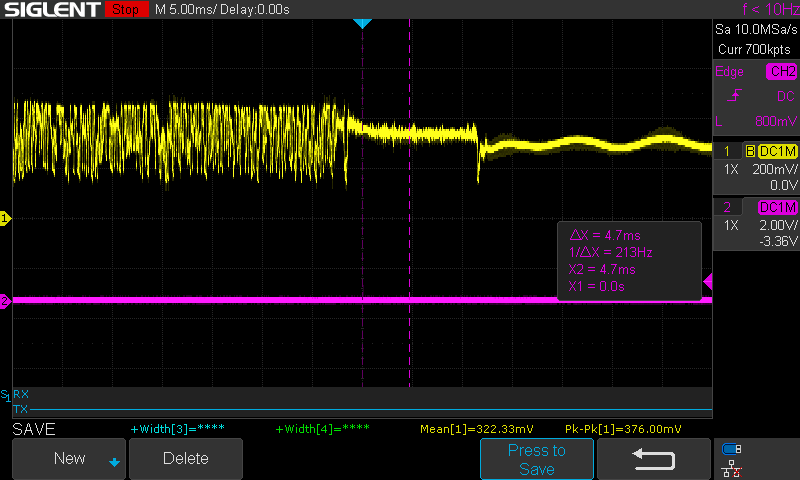
\includegraphics[width=0.5\textwidth]{First_Working_Capture_Oscilloscope.png}}
    \caption{FT-3D keyup recorded on Siglent SDS1204X-E oscilloscope, triggered using FPGA. The trigger signal on channel 2 (the purple signal) is barely visible as an impulse in the middle of the display.}
    \label{keyup_oscilloscope}
\end{figure}

\begin{figure}
    \centerline{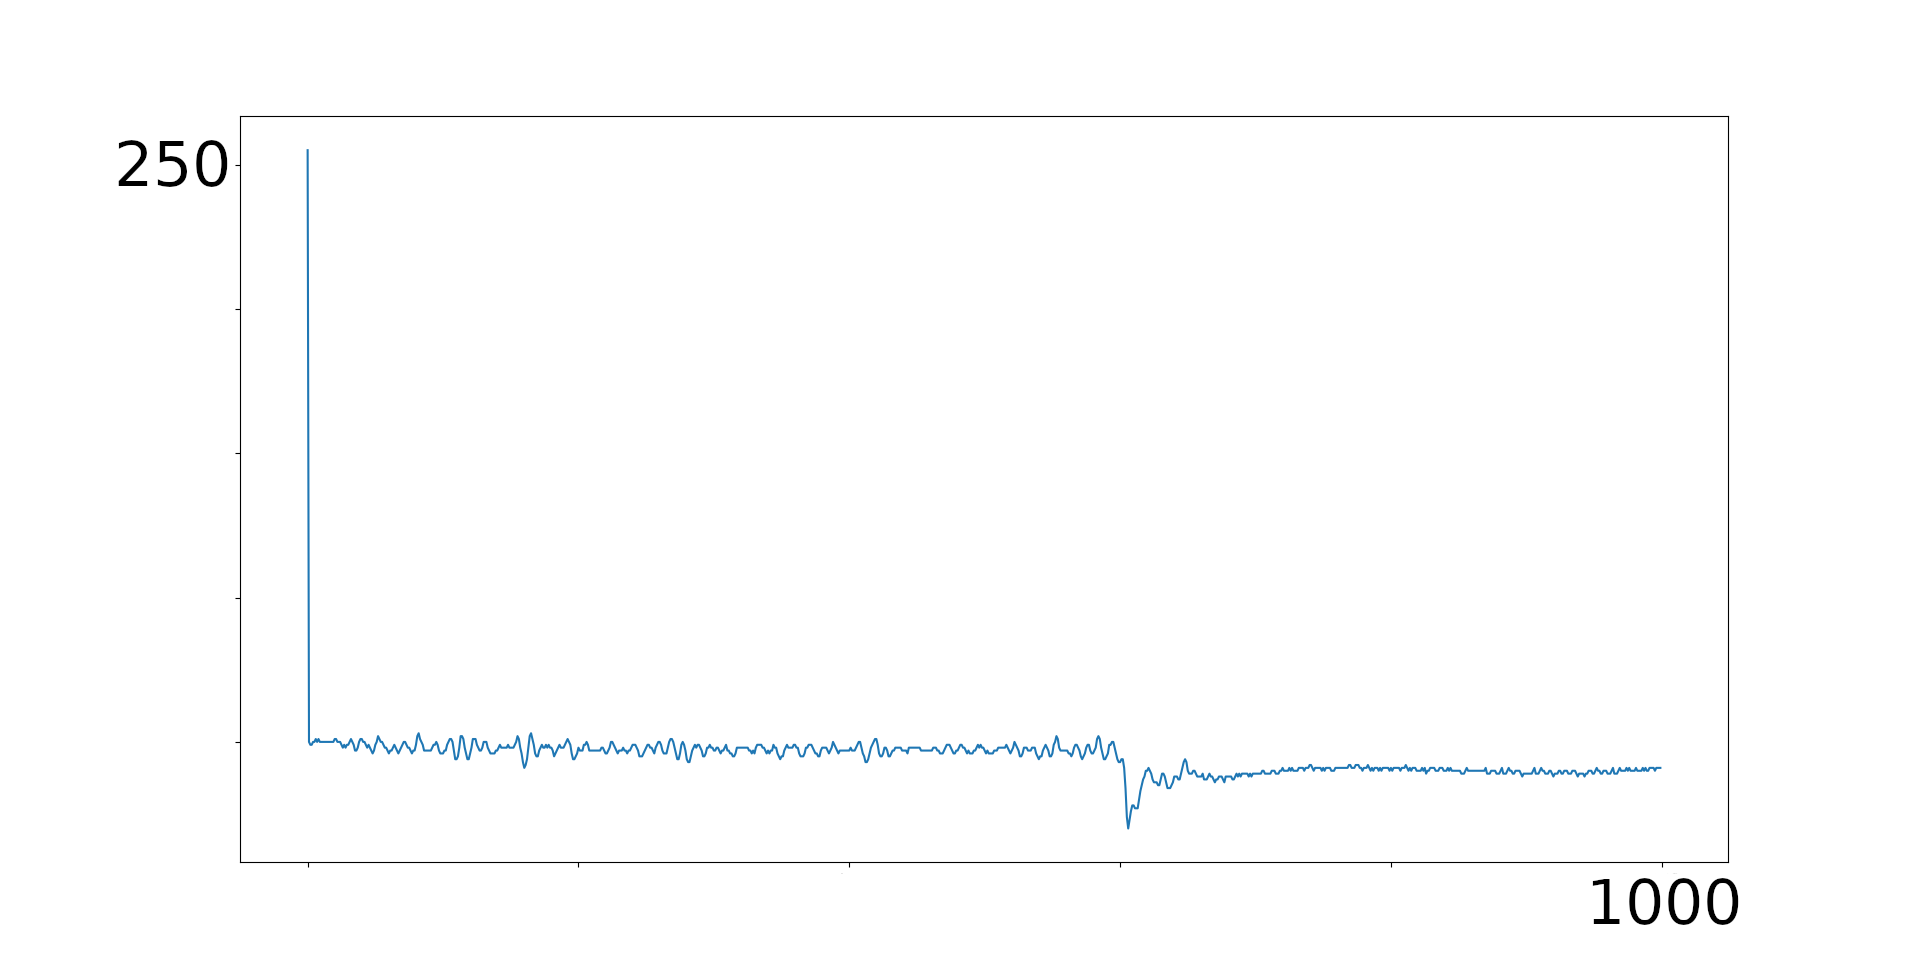
\includegraphics[width=0.5\textwidth]{First_Working_Capture_FPGA.png}}
    \caption{FT-3D keyup recorded on FPGA and exported over UART to computer. Note the similar characteristic ``triple decaying peaks" feature of this radio visible in both the oscilloscope and FPGA captures.}
    \label{keyup_fpga}
\end{figure}

\subsection{Matched Filtering}

In the original design, the matched filter modules performed a simple correlation between the incoming signal and a stored fingerprint signal by sliding one across the other and computing their dot products at each point. The correlation score would be the maximum dot product. Since correlations require a zero-mean signal, the stored fingerprint is preprocessed by a Python script to subtract out an DC bias. The incoming waveform must be averaged (and that average subtracted from the sample values to produce signed values from unsigned ones) by the matched filter module.

This method produced reasonable results but frequently had issues with signals of very different magnitudes, as the dot product of a very strong fingerprint against a completely differently-shaped but weaker signal is still a fairly large number. To combat this, we added a second stage that aligns the fingerprint and the signal using the phase shift determined by the location of the maximum dot product, then computes the sum of the squared differences between the waveforms. This produces a ``similarity score" which is dramatically \emph{lower} for matching waveforms than for non-matching ones. See Fig~.\ref{python_matching} for examples. The blue and orange waveforms are the fingerprint and signal being compared against (aligned in time using the phase shift determined by the matched filtering). The green waveforms show the squared difference between those waveforms. As you can see, the green waveform will be near zero for signals that are actually similar but very spiky for signals that have different shapes.

With the new algorithm, selecting the match becomes trivial--the lowest similarity score is the match. Similarity scores tend to be orders of magnitude different between matches and non-matches, so there is little ambiguity.

\subsection{External Buses}

Simple FSMs implemented SPI and UART buses for communicating with the ADC, communicating with the microSD card, outputting final match scores, and outputting signal traces to a computer. We also used the LEDs to indicate detected radios' identities for rapid testing in hardware.

\subsection{Internal Buses}

All the internal modules communicate using AXI, sometimes augmented with ``trigger" signals for the start of an event. The SPI and UART controllers also use an ``axiready" signal to indicate when they have finished sending a byte and are ready for another.

\subsection{microSD Card Controller}

Building a more robust microSD card controller was a side goal of this project, since the one currently in use by the course can only communicate with SDSC cards (8MB-2GB size). The initialization protocol of microSD cards, apart from being proprietary and largely unknown, is complex enough that implementing it in a pure hardware FSM would be unwieldy and a poor use of resources.

Instead, we chose to make a small softcore CPU with a 16-instruction ISA, instruction ROM, 11 registers, and a simple Python-based assembler. The ISA is tailored towards easy communication with an SD card, including single instructions that perform SPI transactions or issue SD card commands with the appropriate CRCs and formatting. The system can correctly initialize both a 2GB and an 8GB card (reading from an 8GB card requires changing a mode in the firmware to use use block addresses instead of direct addresses, as larger cards addresses are ``divided by 512").

The CPU also has basic arithmetic and bitwise instructions, the ability to load and store constants, the ability to display error codes on the FPGA dev board's LEDs, conditional/branching instructions, and the ability to control the clock select line of the SPI bus directly (because SD cards need mildly non-standard CS manipulation to work correctly).

The CPU does not have or need any RAM, only a ROM containing a program that it starts executing after reset. The program is generated by a Python script that acts as a simple ``assembler," where calling Python methods of an Assembler object causes it to write out binary to a file that is then converted into a .memh file for Vivado. The entire FSM for initializing and reading blocks from a microSD card takes 144 32-bit instructions.

\subsubsection{Development and Debugging of the microSD Controller}

No freely-available or iVerilog-compatible simulation model of a microSD card in SPI mode exists anywhere that we could find online, so debugging had to be done in-situ. We verified the correct operation of the CPU itself in simulation using test programs that did not require a real card to interact with. Then, we wrote Verilog to mirror all the SPI communication lines to the card out to the JC Pmod connector on the dev board, then connected an inexpensive fx2lafw-based 24 MHz USB logic analyzer to those GPIO pins and used Pulseview to record the entire initialization and reading sequence.

Pulseview has the ability to decode both SPI and the higher-level SD card protocol built on top of it, as well as identifying errors and extrapolating the internal state of the card based on that data. Fig.~\ref{pulseview} shows an actual example capture and decode of the start of a successful initialization of an 8 GB Netac microSD card. Mousing over the different parts of the decoded waveform diagram in Pulseview shows what each individual bit in the card's response means, which was extremely useful in debugging issues with the internal state of the card that would otherwise be completely opaque.

Official documentation of the microSD card protocol is not available online without buying a license, but we were able to base the card controller firmware off of the behavior of the Arduino SD card library \cite{b4}, which has been extensively tested on many cards.

We also used a remarkably detailed website about the general architecture of the SD card protocols that purports to originate from an anonymous cat known as ChaN in Japan who works as an embedded engineer \cite{b2}. This website gave us the critical piece of information for initializing \textgreater 2GB cards--that some cards use the ACMD41 sequence for initialization but others use the CMD1 sequence. Trying both is required to cause all cards to initialize successfully. The SD card controller firmware accounts for this, trying one sequence until a timeout is reached, then trying the other.

We also adapted ideas from a previous personal project called OliverRISC (a CPU that could load its program from an SD card). The ISA of the SD card controller is much more specialized than that of OliverRISC, but the firmware implements a similar protocol. The firmware had to be completely rewritten because OliverRISC has actual RAM and a stack, whereas the SD card CPU only has registers.

\begin{figure}
    \centerline{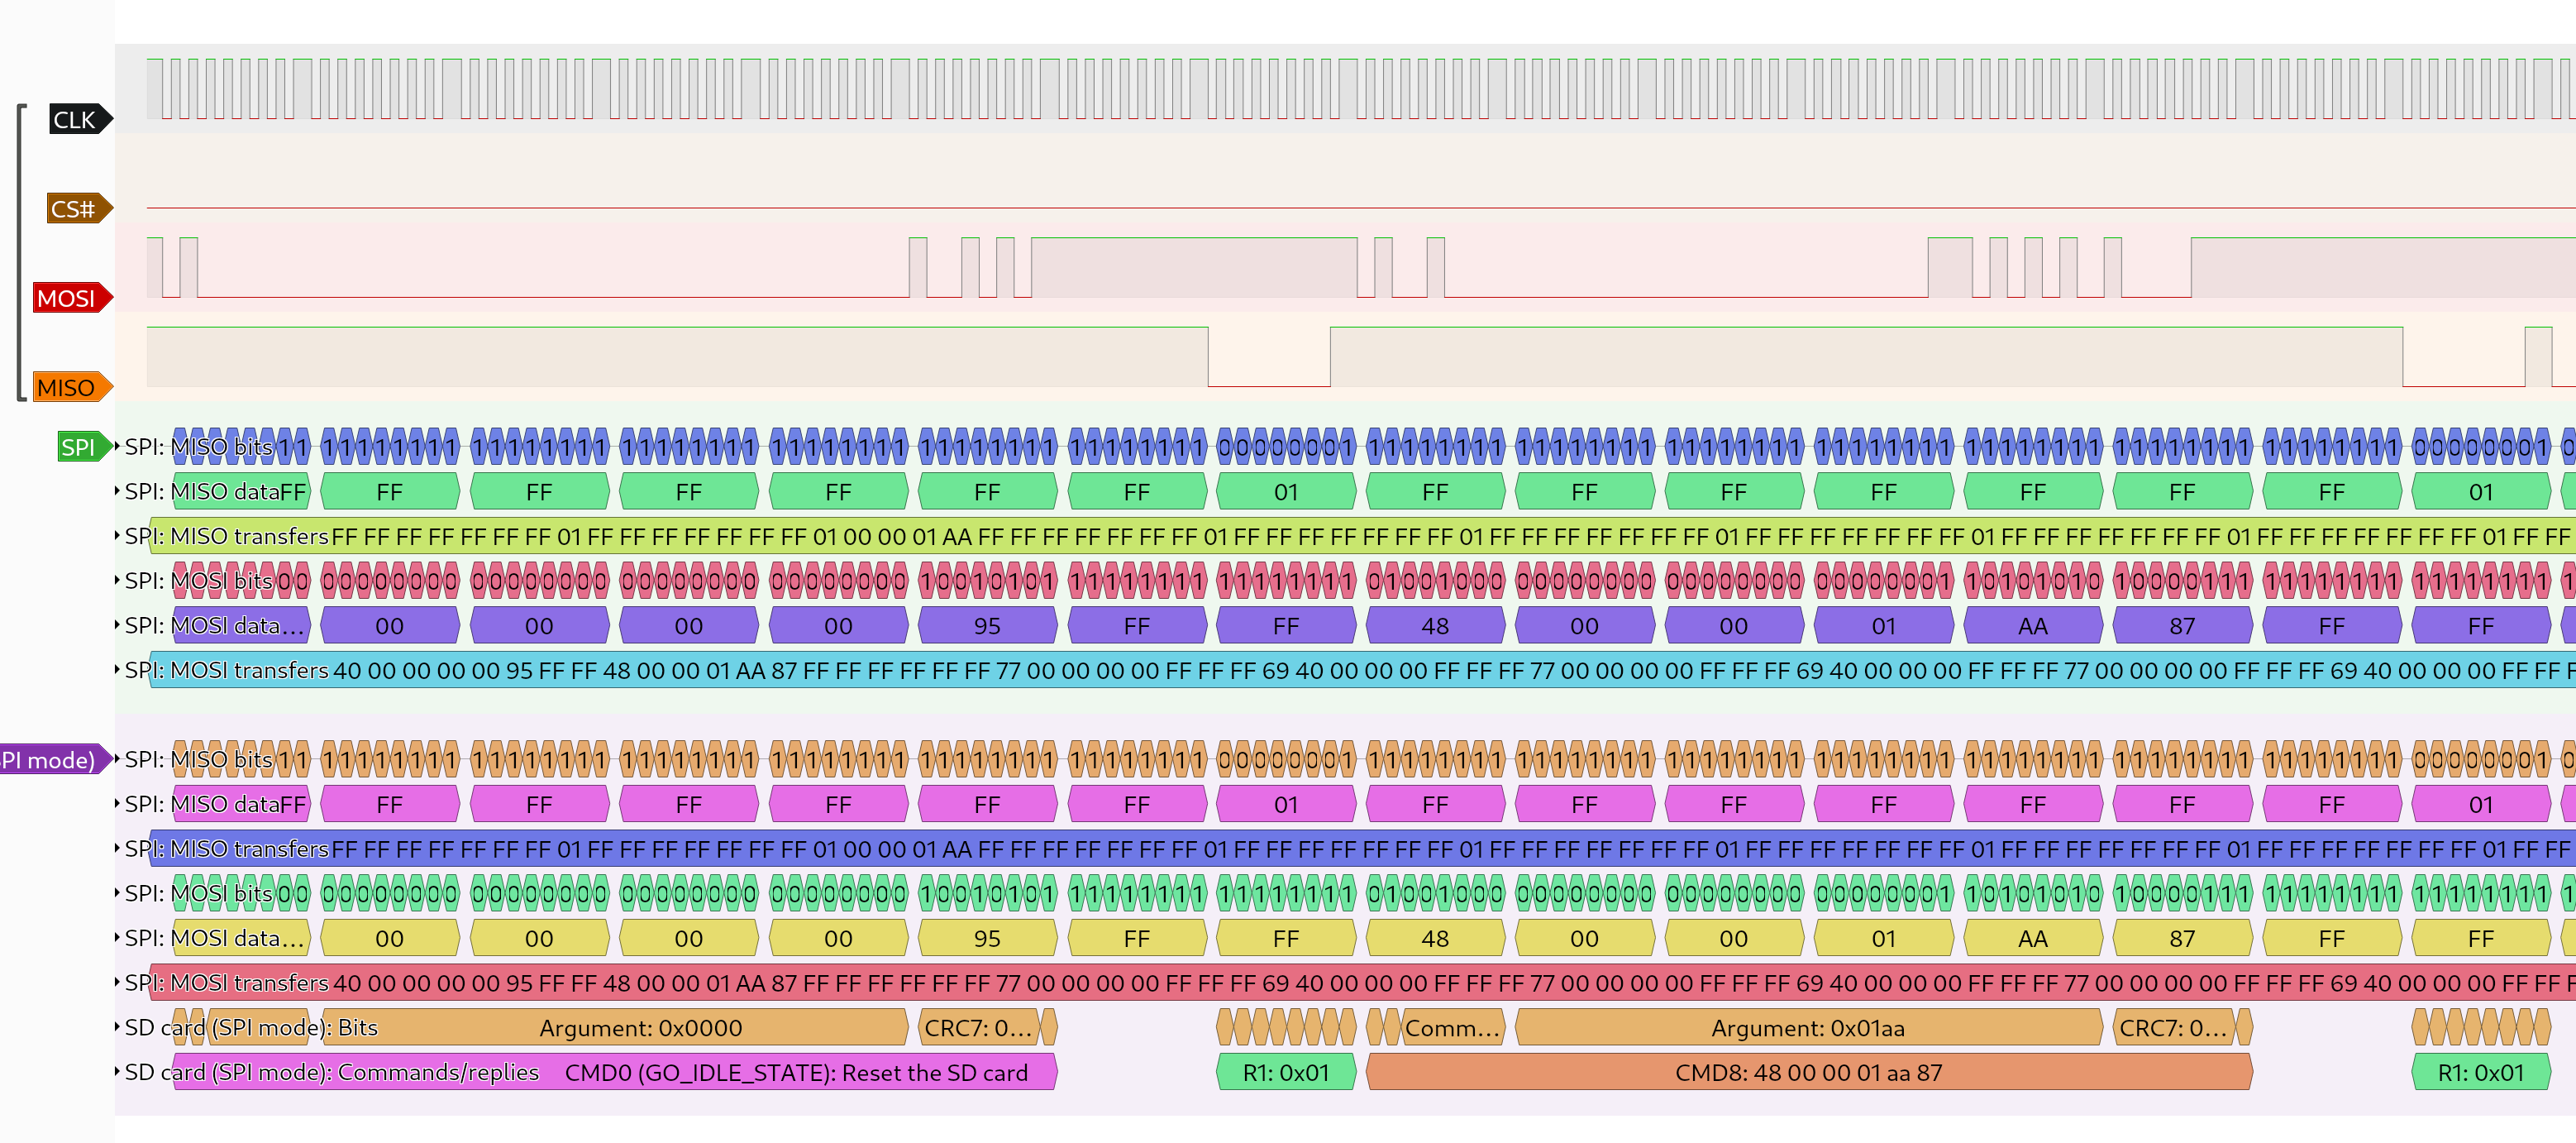
\includegraphics[width=0.5\textwidth]{Pulseview.png}}
    \caption{Pulseview decoding the beginning of the initialization sequence of an 8 GB microSD card from Netac}
    \label{pulseview}
\end{figure}

\section{Evaluation Results}

The matched filters correctly load and classify between FT-3D and FT-70D keyups reliably in hardware (see project video). Using the match scores dumped via a debug SPI port created in the filter manager, we see that the FT-3D matched filter outputs a similarity score around 4000-8000 when an FT-3D keys, whereas the FT-70D matched filter outputs a score around 70000 (lower similarity score means more similar, see section on matched filtering). Conversely, when an FT-70 keys up, the FT-3D matched filter outputs a score around 101000, whereas the FT-70 matched filter outputs around 31000.

Additionally, Python emulation of the matching algorithms used in the FPGA let us gain more insight into the internals of the filtering (see Fig.~\ref{python_matching}).

One of the major goals of this project was to push the total number of matched filters we can instantiate while fitting within the FPGA's resources. We managed to get to 10 filters before being stopped by timing issues caused by Vivado's inability to infer pipelining for the DSP48 slices unless the user explicitly instantiates them (something we could not do because there is no unencrypted Verilog simulation model of a DSP48 slice, so we would've been forced to migrate to Vivado's simulator in the last week of the project).

The design works at the original planned clock speed of 100 MHz. It very slightly does not meet timing at this speed (WNS = -0.234), but does appear to work reliably in the specific hardware we have up to about 10 matched filters being instantiated (this was determined with actual testing in hardware). This could be easily fixed if we could enable the DSP48 pipelining explicitly.

It takes a matched filter around 40 ms to receive a capture (measured using simulation), perform a correlation to determine the appropriate phase shift, and calculate a similarity score by finding the mean squared difference between the signals. This is well within the time before somebody generally starts talking into their radio after keying it up, so we have enough margin to have time left over for the slower SPI bus to send the match data to a repeater controller or computer (in a future design, this final output could probably also be replaced with a faster bus like PCIe or Ethernet).

Everything is fully-pipelined (although, as mentioned elsewhere, Vivado struggles to fit an entire DSP48 multiply into one clock), so the throughput is 1 sample per clock cycle.

The design uses 2 DSPs and 1 BRAM per matched filter. For reasons that remain unclear, the DSP utilization report always reports 4 DSPs being used, regardless of how the design is changed, even though the actual synthesis log (and the behavior in hardware one we add more filters than the timing can handle) definitely shows that adding more matched filters to the code causes them to be synthesized. Once again, we suspect that using the Vivado simulator earlier on in the project and explicitly controlling DSP48 usage/pipelining would help.

The design could be improved to use only 1 DSP per matched filter, since the only reason there are 2 is that Vivado creates separate multipliers for different states of the FSM that never actually run at the same time. However, attempting to separate out the multiplier to stop this behavior causes Vivado to not infer a DSP48 slice at all.

General logic utilization (LUTs) was very low at only 3.12\% of Slice LUTs, since most of the resource usage is in BRAMs and multipliers. Most of that logic is probably going to the debug and SD card interfaces. The synthesizer struggles with congestion due to the large fanout of many parallel filters but manages to resolve it after a few attempts.

One of the large overheads incurred is the time and logic spent on effective debugging systems (most of which could be switched off in a final product to save logic). Most buses slow enough for the oscilloscope or logic analyzer to read accurately over long wires are slower than the actual operating speed of the logic, so buffers are required to run them. UART is extremely slow and requires an extra FSM, so exporting signals to a computer takes time. The SPI bus used to output match scores is also fairly slow, which, in actual use, would decrease the amount of time the repeater controller has to react to a blocked user detection. However, these tools made developing the system a lot easier, as they all offer windows into parts of the actual DSP chain that let us debug the system more effectively.

The design is definitely usable for the use case of detecting and locking out a single user and could trivially be extended to the use case of detecting/logging multiple users of a repeater for some kind of ``scoreboard" system.

With minimal changes, the design could also be extended with a CAT (Computer Aided Transceiver) interface back to the radio (usually just an RS-232 port) that would allow it to scan multiple frequencies and build up a general summary of who is transmitting on the air throughout the day.

With much larger changes, the design could be used on an FPGA with an SDR interface like the HackRF so that it could fingerprint and identify all users within a slice of RF bandwidth at the same time, creating a valuable tool for analyzing interference sources or characterizing user behavior.

\begin{figure}
    \centerline{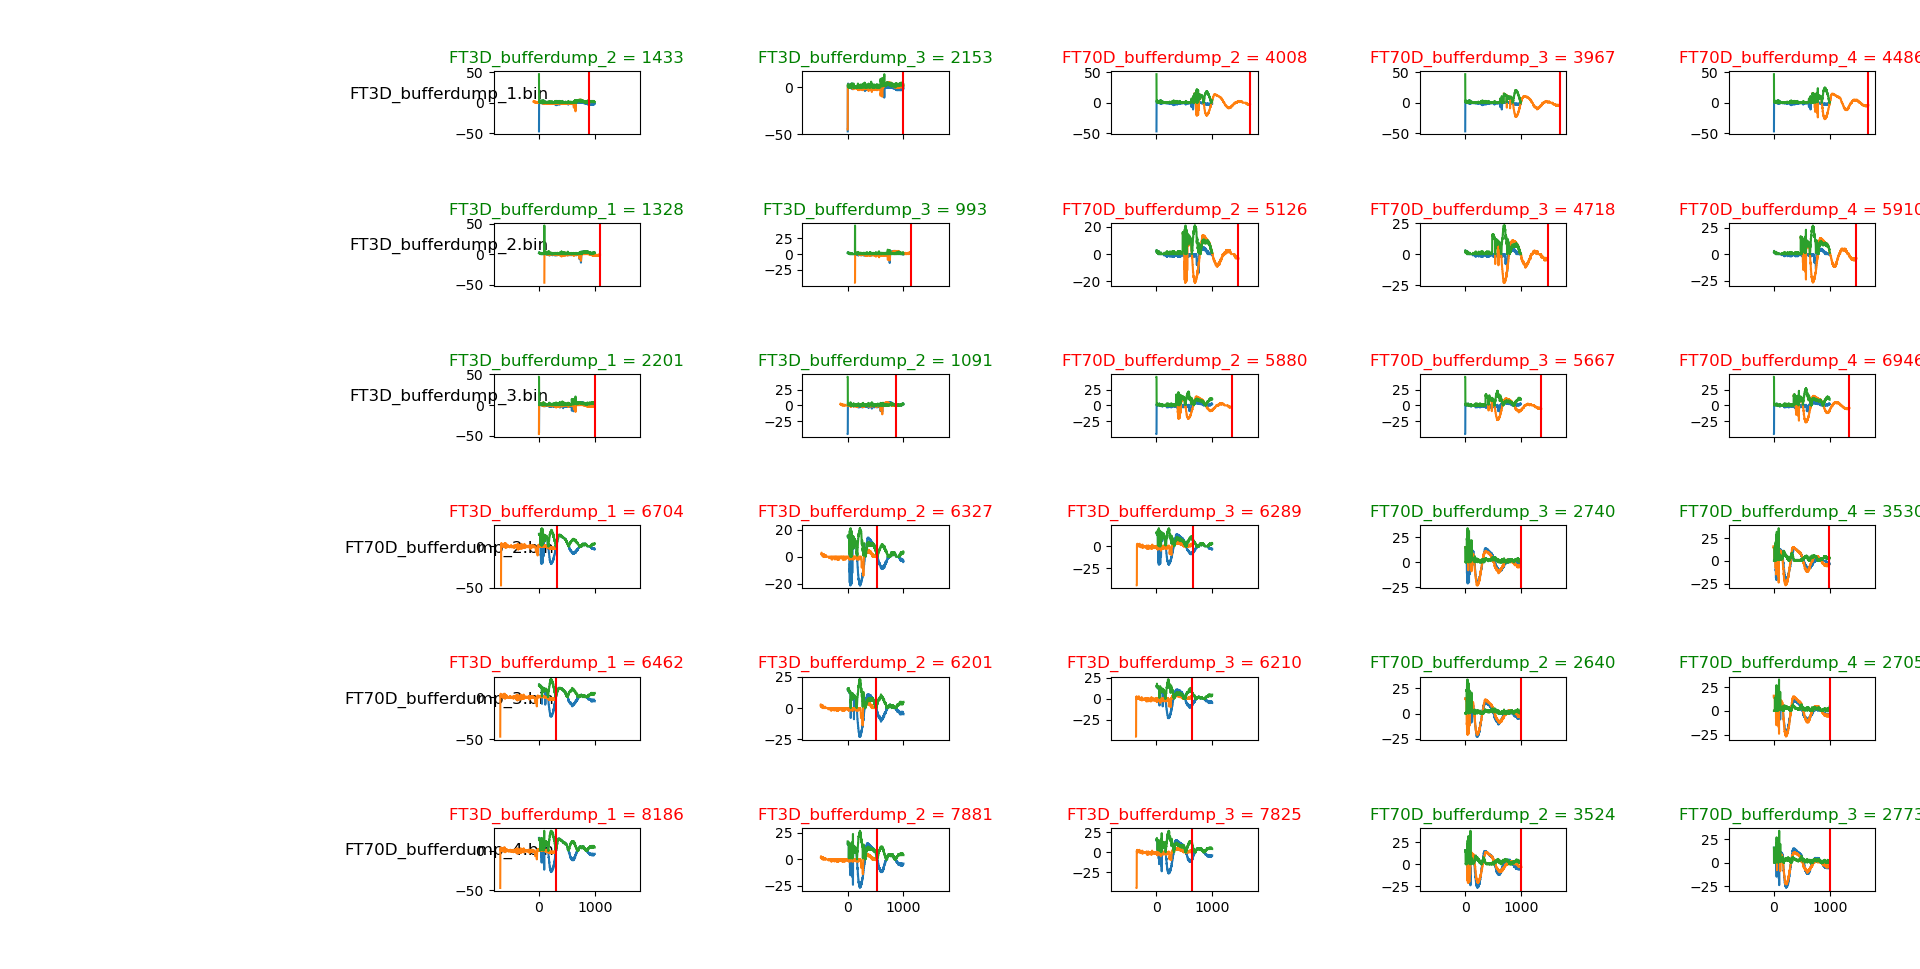
\includegraphics[width=0.5\textwidth]{Successful_Classifications.png}}
    \caption{Python emulation of comparing different FT-3D and FT-70D fingerprints against each other. Black text on the left edge shows which fingerprint that row of graphs was compared against. Colored text above each graph shows which other signal that comparison was run against. Green and red show matches and non-matches.}
    \label{python_matching}
\end{figure}

\begin{figure}
    \centerline{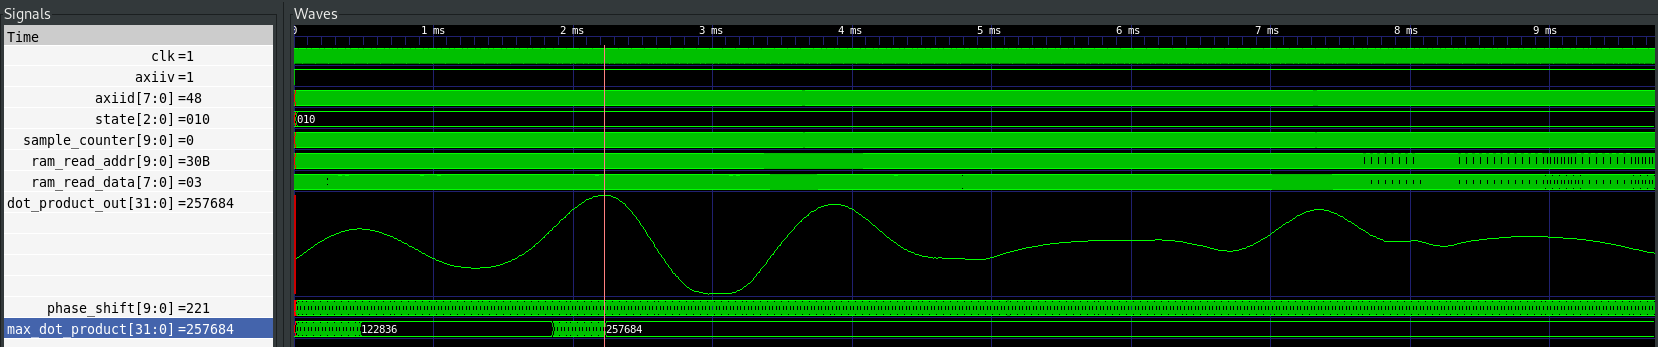
\includegraphics[width=0.5\textwidth]{FT70D_vs_FT3DR.png}}
    \caption{GTKWave visualization of output of matched filter correlating a reference fingerprint of an FT-70D radio against an FT-3DR. The \lstinline{dot_product_out} signal shows the correlation waveform.}
    \label{correlation}
\end{figure}

\section{Instrumentation and Testing}

We used a Siglent SDS1204X-E digital storage oscilloscope to obtain initial recordings of various radios' keyup characteristics to develop the matched filtering in Python and determine what sampling rate/bit depth would be required to accurately reproduce the signals. A custom C program from a previous project for converting oscilloscope binary dump files into CSV files was extremely useful.

We also used a Siglent SDG2042X arbitrary waveform generator to generate repeatable test waveforms to ensure that the ADC was digitizing incoming signals correctly.

A Python script that recorded and stored exported signals from the FPGA's UART over an FTDI cable allowed us to easily run testbenches in Icarus Verilog against the exact signals as the FPGA would see them. This was extremely useful for verifying and debugging DSP algorithms. Additionally, it allowed us to generate ROMs of actual fingerprint signals and synthesize them into the design's matched filtering stage for testing the filters without having to load the data from the microSD card.

Most of the DSP algorithms were prototyped in Python and C both to develop them more easily and to provide a reference implementation to compare the output of Verilog testbenches to.

Each module in the design had its own testbench (some which used \lstinline{$readmemh()} to load memory files generated from actual recorded signals from the UART), as well as small Bash scripts to run the testbenches and open GTKWave with the appropriate display configuration. We used GTKWave's ``analog waveform display" option extensively to display register values as smooth waveforms for easy visual debugging of DSP algorithms.

Pulseview's protocol analysis/decoding tools and Sparkfun's 24 MHz USB logic analyzer, as discussed previously, were critical to being able to develop a working SD card controller without a working simulation model of an SD card.

\section{Insights and Next Time}

The project completed its goals and, due to the ``similarity score" algorithm we came up with in the final weeks of the project, outperformed our initial expectations of reliability based on the early C/Python code written to test the DSP chain.

However, if we were to do this again, we would set up the project to use XSim, Vivado's own internal simulator, from the beginning. This would alleviate issues with suble differences in signed number handling and, more importantly, allow us to simulate direct use of the DSP48 slices. The Vivado wizard for creating a DSP48 instantiation actually allows users to directly customize the exact pipelining inside the slice, which would have been incredibly useful and likely allowed us to solve the timing issues and run somewhere in the neighborhood of 100 parallel filters easily.

\section{Code}

GitHub repo containing all Verilog code, as well as the toolchain and firmware for the SD card controller (and some C/Python code for DSP testing):

https://github.com/featherfeet/6111\_Final\_Project

\begin{figure*}
    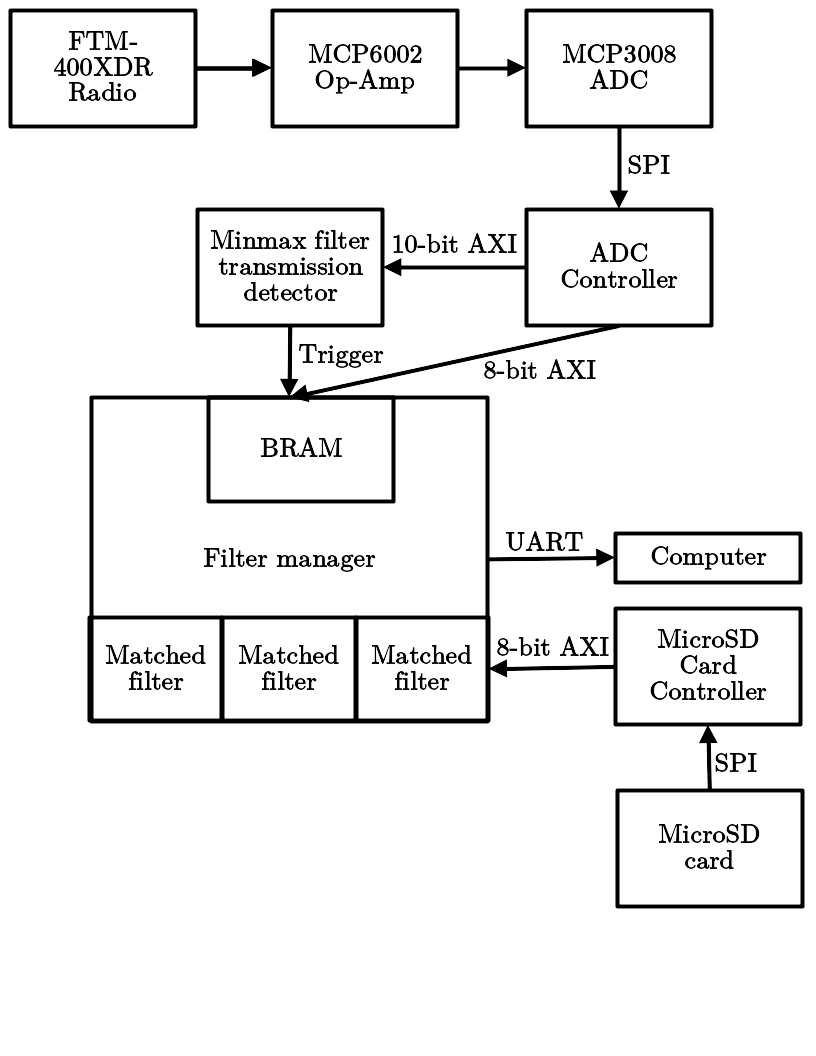
\includegraphics[width=\textwidth]{Block_Diagram.png}
    \caption{Full system block diagram}
    \label{block_diagram}
\end{figure*}

\begin{thebibliography}{00}
\bibitem{b1} B. Fields, ``Transmitter fingerprinting," \emph{W9CR}, 19-Nov-2020. [Online]. Available: https://wiki.w9cr.net/index.php/Transmitter\_Fingerprinting. [Accessed: 23-Nov-2022].

\bibitem{b2} ChaN, ``How to use MMC/SDC," \emph{ELM-CHAN}, 26-Dec-2019. [Online]. Available: https://users.ece.utexas.edu/~valvano/EE345M/view12\_SPI\_SDC.pdf. [Accessed: 09-Dec-2022].

\bibitem{b3} R. Rager, ``XMIT\_ID version 2.61," XMIT ID version 2.61, 15-Nov-2000. [Online]. Available: https://www.qsl.net/n9zia/xmit\_id/index.html. [Accessed: 23-Nov-2022].

\bibitem{b4} Arduino Project Authors, ``SD Library for Arduino," \emph{GitHub}, 12-Nov-2022. [Online]. Available: https://github.com/arduino-libraries/SD. [Accessed: 09-Dec-2022].
\end{thebibliography}

\vspace{12pt}

\end{document}
